%
% 01_NWP.tex -- Beispiel-File für das Paper
%
% (c) 2023 Dmitry Grigoriev, OST Ostschweizer Fachhochschule
%
% !TEX root = ../../buch.tex
% !TEX encoding = UTF-8
%
\section{Numerische Wettervorhersage
\label{spektral:section:nwp}}
\rhead{Numerische Wettervorhersage}
Die numerische Wettervorhersage ist ein entscheidendes Instrument in der modernen Meteorologie. Durch die Anwendung von mathematischen Gleichungen, physikalischen Gesetzen und Computermodellen ermöglicht sie die Vorhersage von zukünftigen Wetterbedingungen. Hierbei werden umfangreiche Daten wie Temperatur, Luftdruck, Feuchtigkeit und Windgeschwindigkeit von verschiedenen Messstationen weltweit gesammelt und in hochentwickelte Computermodelle eingespeist.

In diesem Abschnitt werden wir die Gittermodelle und die spektrale Modelle anschauen. Im Abschnitt \ref{spektral:subsection:spektralemodelle} werden wir die spektrale Modelle an die Wellengleichung anwenden, um die Vorteile solchen modellen zu zeigen.

\subsection{Finite-Difference-Gittermodelle
\label{spektral:subsection:gittermodelle}}
In den meisten Fällen ist die Lösung von partiellen Differentialgleichungen nur mithilfe von numerischen iterativen Methoden möglich. 
Die Idee dieser Methoden besteht darin, die Differentialgleichungen zu diskretisieren.
Die Ableitungen werden durch finite Differenzen dargestellt.
Dadurch können die Differentialgleichungen in algebraische Gleichungssysteme umgewandelt werden.
D.h. es werden die Werte der Variablen nicht für die gesamte unendliche Menge von Punkten im Bereich untersucht, sondern nur für eine endliche Teilmenge.

Die Methode der endlichen Differenzen beinhaltet die Diskretisierung von Funktionen auf einem Gitter.
In diesem Fall sind die Werte der Funktion die Knoten des Gitters und Ableitungen werden durch endliche Differenzen ersetzt.

Vorwärtsdifferenz:
\begin{equation}
\frac{du}{dt} = \frac{u(t + \Delta{t}) - u(t)}{\Delta{t}}.
\label{spektral:equation1}
\end{equation}

Rückwärtsdifferenz:
\begin{equation}
\frac{du}{dt} = \frac{u(t) - u(t - \Delta{t})}{\Delta{t}}.
\label{spektral:equation2}
\end{equation}

Zentraledifferenz
\begin{equation}
\frac{du}{dt} = \frac{u(t + \Delta{t}) - u(t - \Delta{t})}{2\Delta{t}}.
\label{spektral:equation3}
\end{equation}

Üblicherweise werden Diskretisierungsgitter gewählt, die mit den Koordinatengittern übereinstimmen.
In einem zweidimensionalen kartesischen Koordinatensystem die Gitterzellen sind die Rechtecke.
\pagebreak
\begin{figure}[h]
	\centering
	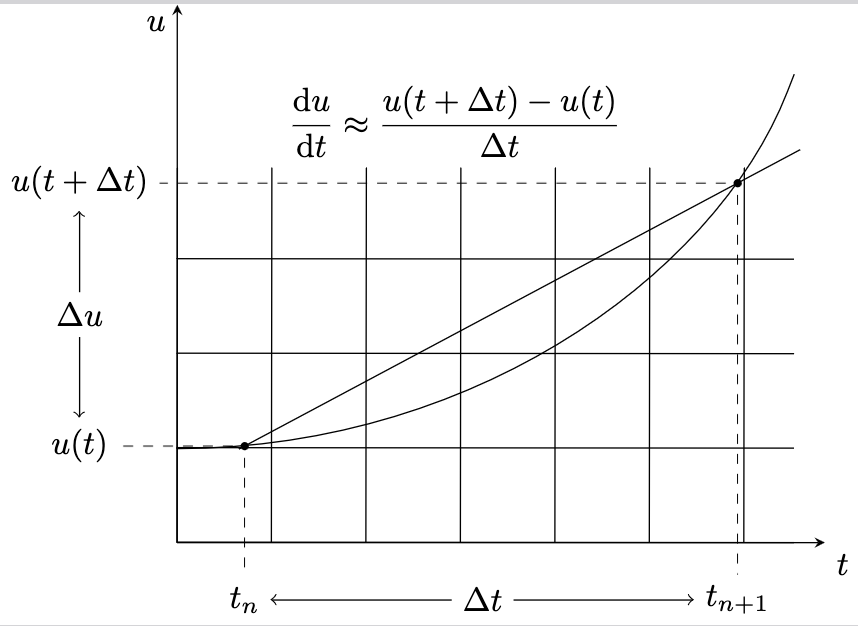
\includegraphics[height=180pt]{papers/spektral/images/forwarddiff.png}
	\caption{Vorwärtsdifferenz}
    \label{spektral:fig:gittermodelle}
\end{figure}

Auf der Abbildung \ref{spektral:fig:gittermodelle} sieht man, dass für eine Funktion mit einer Variable werden viele Punkte für die Vorhersage benötigt. Für die Funktion der 3 Variablen werden die Millionen von Datenpunkten und, damit man eine gute Wetterprognose mit der Methode machen kann, werden höhe Rechnungsleistungen benötigt.

\subsection{Was sind die spektrale Modelle?
\label{spektral:subsection:spektralemodelle}}
In den 1980er Jahren des 20. Jahrhunderts wurden neben den gitterbasierten (Finite-Difference) Lösungsmethoden, die traditionell in Vorhersagemodellen verwendet wurden, auch Methoden angewendet, bei denen die räumliche Abhängigkeit der prognostizierten meteorologischen Werten als Reihen von Funktionssystemen dargestellt wird, die bestimmte Eigenschaften aufweisen.

In diesem Fall wird die prognostizierte Gleichung oder das System von partiellen Differentialgleichungen auf Systeme von Differentialgleichungen für die zeitabhängigen Koeffizienten der Zerlegung reduziert.
Die gesuchte Werte bei diesem Ansatz sind diese Koeffizienten und nicht die Werte der prognostizierten Funktionen an den Gitterpunkten. 
Eine Variante dieser Methode im Bereich der numerischen Wettervorhersage wird als spektrale Methode bezeichnet und Vorhersagemodelle, bei denen die Gleichungen mit der spektralen Methode gelöst werden, werden als spektrale Modelle bezeichnet.

Spektrale Modelle sind eine Art numerischer Modelle, die in verschiedenen wissenschaftlichen Bereichen, einschließlich der Meteorologie, verwendet werden.
Diese Modelle basieren auf der Verwendung spektraler Methoden, um mathematische Gleichungen, die physikalische Phänomene beschreiben, zu lösen.

In der Meteorologie beziehen sich spektrale Modelle auf Vorhersagemodelle, die spektrale Methoden verwenden, um atmosphärische Prozesse zu simulieren und Wettervorhersagen zu erstellen.
Anstatt die Erde und die Atmosphäre in einem diskreten Gitter zu modellieren, wie es bei gitterbasierten Modellen der Fall ist, verwenden spektrale Modelle eine Fourier-Transformation, um die Atmosphäre in eine Kombination von Wellen mit verschiedenen Frequenzen aufzubrechen.
Dies ermöglicht es, die Atmosphäre kontinuierlich und mit höherer Auflösung zu modellieren.

Insgesamt sind spektrale Modelle ein wichtiger Ansatz, um detaillierte Einblicke in atmosphärische Prozesse zu gewinnen und präzise Wettervorhersagen zu erstellen, insbesondere wenn es um die Wellen und die Schwingungen geht.

\subsection{Vorteile der spektralen Modellen
\label{spektral:subsection:vorteile}}

\begin{itemize}
\item
\textbf{Genauere Erfassung von Wellenphänomenen:} Spektrale Modelle sind besonders gut darin, atmosphärische Wellenphänomene wie Schallwellen, Rossby-Wellen und atmosphärische Oszillationen zu erfassen.
Sie können die räumliche Ausbreitung und Interaktion dieser Wellen genau simulieren.
\item
\textbf{Bessere Darstellung von großen und kleinen Skalen:} Spektrale Modelle haben eine hohe räumliche Auflösung, die es ermöglicht, sowohl großräumige globale Muster als auch kleinräumige lokale Effekte detailliert zu modellieren.
Dadurch können sie sowohl makroskalige als auch mikroskalige Phänomene abdecken.
\item
\textbf{Konsistente Erhaltung bestimmter Größen:} Spektrale Modelle haben oft eine bessere Erhaltung von Energie, Impuls und anderen wichtigen physikalischen Größen.
Dies trägt zur Erzielung physikalisch konsistenterer Simulationen bei.
\item
\textbf{Effiziente Modellierung periodischer Phänomene:} Spektrale Modelle sind gut geeignet zur Modellierung periodischer Phänomene, da sie periodische Signale genau erfassen können, ohne hohe räumliche Auflösung überall zu erfordern.
\item
\textbf{Reduzierter Diffusionseffekt (Rauschresistent):} Im Vergleich zu einigen gitterbasierten Methoden, die zur Stabilisierung numerischer Instabilitäten künstliche Diffusion einführen müssen, weisen spektrale Modelle oft einen geringeren Diffusionseffekt auf, was zu genaueren und detaillierteren Simulationen führen kann.
\item
\textbf{Adaptivität und Flexibilität:} Spektrale Modelle können auf verschiedene Geometrien und Randbedingungen angewendet werden und sind nicht auf regelmäßige Gitterstrukturen beschränkt.
Dies ermöglicht eine höhere Anpassungsfähigkeit an komplexe Geländeformen.
\item
\textbf{Einfachere Lösung:} Spektrale Modelle führen auf viel einfachere algebraische Gleichungen.
\end{itemize}

\subsection{Kugelkoordinaten
\label{spektral:subsection:kugelkoordinaten}}

Bevor wir die spektrale Modelle nähe anschauen, müssen wir die von den kartesischen Koordinaten zu den Kugelkkordinaten wecheln, weil wir uns auf einer Kugel befinden (siehe Abbildung \ref{spektral:fig:sphericalcoords}).

\begin{figure}[h]
	\centering
	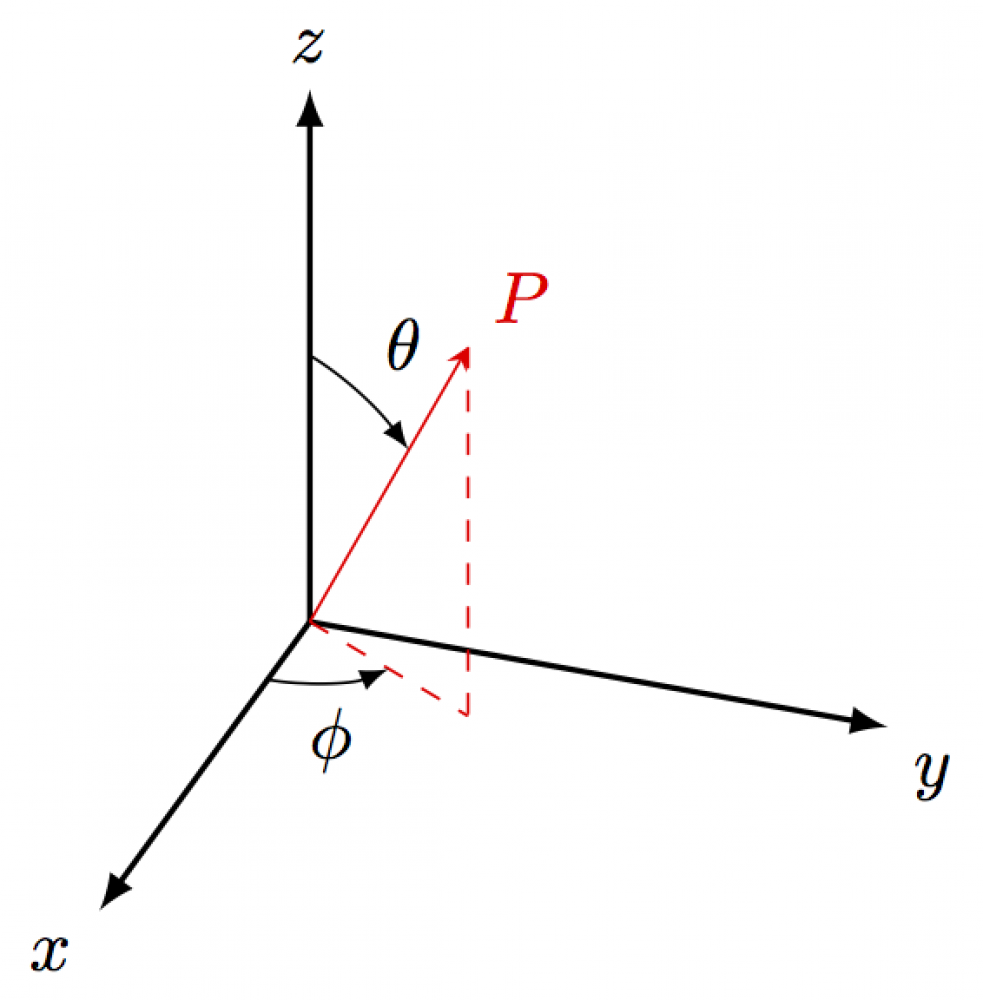
\includegraphics[height=120pt,width=120pt]{papers/spektral/images/spherical_coordinates.png}
	\caption{Sphärische Koordinaten}
    \label{spektral:fig:sphericalcoords}
\end{figure}
\pagebreak

\begin{align}
x &= r\cdot\sin(\theta)\cdot\cos(\phi)
\label{spektral:equation4}
\\
 y &= r\cdot\sin(\theta)\cdot\sin(\phi)
\label{spektral:equation5}
\\
 z &= r\cdot\cos(\theta).
\label{spektral:equation6}
\end{align}
wobei $r > 0$ sein muss, sonst können $\theta$ und $\phi$ nicht definiert werden.


